\documentclass[a4paper, 12pt,oneside]{article}
\usepackage[paper=a4paper,left=30mm,right=25mm,top=25mm,bottom=25mm,includeheadfoot]{geometry}
\usepackage{framed}%this package is the basis for the 'framed'-elements
%\usepackage[ngerman]{babel}
%uncomment the previous line to automatically translate the standard-elements to german. Otherwise they will be in english
\usepackage{amsmath}
\usepackage{mathtools}
\usepackage{amsfonts}
\usepackage{amssymb}
\usepackage{graphicx}
\usepackage{dtklogos}% enables writing BibTeX in its special notation and similar symbols. not needed for TeX and LaTeX special writing styles
\usepackage[utf8]{inputenc}
\usepackage[T1]{fontenc}
\usepackage{setspace}
\usepackage{hyperref}
\usepackage[acronym]{glossaries}%put this line before the hyperref-inclusion to have glossaries without links
\setcounter{tocdepth}{4}
\setcounter{secnumdepth}{4}
\usepackage{color}
\usepackage{datetime}
\usepackage{natbib}%setting for bibliography-integration-package
\bibpunct{(}{)}{;}{a}{,}{,}

%the basics for theorems, definitions and lemmata
%more info on http://en.wikibooks.org/wiki/LaTeX/Theorems
%even more on http://www.math.uiuc.edu/~hildebr/tex/tips-theorems.html
\usepackage{amsthm}%used for writing theorems
\usepackage{thmtools}%also used for writing theorems
\declaretheorem{theorem}
\declaretheorem[style=definition]{definition}
\declaretheorem{example}


\usepackage[final]{pdfpages}%enables PDF-inclusion
\usepackage{chngcntr}
\counterwithin{table}{section}
\counterwithin{figure}{section}%captions in tables and figures are numbered by the section
%\counterwithin{definition}{subsubsection}

\hyphenation{con-textualize Ent-wurf}% definition for hyphenation-rules. enter the desired hyphenation-style for words to override the defaults. Entries are separated by a space

\begin{document}
\makeatletter
\newcommand{\@Title}[1]{\def\Title{#1}}
\newcommand{\@Student}[1]{\def\Student{#1}}
\newcommand{\@PrimarySupervisor}[1]{\def\PrimarySupervisor{#1}}
\newcommand{\@SecondarySupervisor}[1]{\def\SecondarySupervisor{#1}}


%
%
% Data for your titlepage:
%
%

\@Title{Color palette generator for improved human perception of colors} % The Title of your Thesis goes between the brackets

\@Student{Jay Bhargav Barbhaiya} %your name belongs beween these two brackets

\@PrimarySupervisor{Prof. Dr. Peter Misch} %The full Name AND Title of your primary supervisor belongs between these brackets (It must be one of the Professors at the Department)

\@SecondarySupervisor{Prof. Dr. Gred Moeckel} %The full name and Title of your secondary supervisor belongs in between these two brackets. (That can be anyone - even outside this department - who has the degree you are seeking to obtain: M.Sc. or higher in Computerscience)
%if you chose a secondary supervisor from another company, you are advised to add the name of the company in brackets behind the Supervisors name

%
%
% end of Data for your titlepage
%
%
\makeatother

%
%
% Translation-segment:
%
%

%\renewcommand\listtheoremname{Liste der Theoreme}
%uncomment the previous line to translate the list of theorems to german



%\renewcommand*{\glossaryname}{My new name}
%uncomment the previous line to rename the Glossary

%\deftranslation{Acronyms}{Abkürzungen}
%uncomment the previous line to translate the term Acronyms into the german term 'Abkürzungen'


%
%
% end of Translation-segment
%
%

%\makeglossaries

%
%
% Acronym-definition-segment:
%
%

%entry style is:
%\newacronym{short form as used in the code}{Abbreviation as displayed in the Text}{Description that will appear in the Abbreviation glossary at the end}

\newacronym{cl}{CL}{Cognitive Load}
\newacronym{msc}{M.Sc.}{Master of science}
\newacronym{srh}{SRH}{Stiftung Rehabilitation Heidelberg}

%
%
% end of Acronym-definition-segment
%
%

\hypersetup{pageanchor=false}
\graphicspath{{./img/}} %the folder for the graphics is defined here

\begin{titlepage}
\begin{flushright}

\includegraphics[scale=0.50]{logo_heidelberg_gr.png}
\end{flushright}
\vspace{4em}
\begin{center}



\begin{LARGE}
\textbf{\Title}
\end{LARGE}\\


\vspace{4em}

%\LARGE{Master Thesis} \\


{\LARGE Master Thesis}\\


\vspace{1em}

{\LARGE by}\\

\vspace{1em}
\LARGE{\textbf{\Student}}\\


\vspace{1em}

\newdateformat{mydate}{\monthname[\THEMONTH] \THEYEAR}
{\large {\mydate\today}}\\%automatically writes the date when the Document was finsihed. Comment this line and the above and use the one below to write your own date by hand
%\LARGE{2013-07-11}\\

\vspace{6em}

{\large SRH University Heidelberg}\\
{\large School of Informatics}\\

\vspace{2em}

\end{center}
\makebox{Primary supervisor} \hspace{\fill}\makebox{\PrimarySupervisor}\\
\makebox{Secondary supervisor} \hspace{\fill} \makebox{\SecondarySupervisor}

\vspace*{\fill}
\end{titlepage}
\begin{titlepage}

\begin{flushright}

\includegraphics[scale=0.50]{logo_heidelberg_gr.png}
\end{flushright}
\vspace{4em}
\begin{center}



\begin{LARGE}
\textbf{\Title}
\end{LARGE}\\


\vspace{4em}

%\LARGE{Master Thesis} \\


{\LARGE Master Thesis}\\


\vspace{1em}

{\LARGE von}\\

\vspace{1em}
\LARGE{\textbf{\Student}}\\


\vspace{1em}

\newdateformat{mydate}{\monthname[\THEMONTH] \THEYEAR}
{\large {\mydate\today}}\\%automatically writes the date when the Document was finsihed. Comment this line and the above and use the one below to write your own date by hand
%{\large {2013-07-11}}\\

\vspace{6em}

{\large SRH Hochschule Heidelberg}\\
{\large Fakultät für Informatik}\\

\vspace{2em}

\end{center}
\makebox{Erstgutachter/in} \hspace{\fill}\makebox{\PrimarySupervisor}\\
\makebox{Zweitgutachter/in} \hspace{\fill} \makebox{\SecondarySupervisor}

\vspace*{\fill}
\end{titlepage}
%comment the title_page_EN and uncomment title_page_DE to get the german version

\thispagestyle{empty}%this inserts an empty page between these two

\thispagestyle{empty}
\section*{Affidavit}
Herewith I declare:
\begin{itemize}
\item that I have independently composed the chapters of the Master Thesis for which I am named as the author.
\item that i did not use any other sources and additives but the ones specified.
\item that I did not submit this work for any other examination procedure.
\end{itemize}
\begin{verbatim}





\end{verbatim}
\makebox[0.5\textwidth]{Heidelberg,\enspace\hrulefill}
 
\thispagestyle{empty}
\section*{Eidesstattliche Erklärung}

Ich versichere, dass ich die Kapitel der Arbeit, für die ich als Verfasser genannt werde, selbständig verfasst habe, dass ich keine anderen, als die angegebenen Quellen und Hilfsmittel benutzt habe und dass ich diese Arbeit bei keinem anderen Prüfungsverfahren vorgelegt habe.
\begin{verbatim}






\end{verbatim}
\makebox[0.5\textwidth]{Heidelberg,\enspace\hrulefill}
 
%comment the affidavit_EN and uncomment affidavit_DE to get the german version

% keep in mind: sign the affidavit in handwriting before handing your work in. otherwise

%
%
% Acknowledgements-segment (optional):
%
%

%uncomment the following lines to properly include Acknowledgements in your Thesis in the correct location

%\newpage
%\thispagestyle{empty}
%\begin{center} \begin{LARGE}
%Acknowledgements
%\end{LARGE} \end{center}  
%\vspace{4em}
%you can include the Acknowledgements below here
%I would like to use this occasion to thank...
%\pagebreak

%
%
% end of Acknowledgements-segment
%
%

\thispagestyle{empty}
\hypersetup{hidelinks}
\tableofcontents
\thispagestyle{empty}
\newpage
\thispagestyle{plain}
\setcounter{page}{1}
\pagenumbering{roman}
\onehalfspacing

\begin{center}
{\LARGE Abstract}
\end{center}

Enter your Abstract here. \\
Remember: the abstract is best written as the last part of the thesis after you finsihed everything else. 



Here comes some sample-content to serve as copy-paste material and as a howto-reference for the most common standard-elements. it is located in the 'abstract' section because that is the last section you should write anyway, so the samples can serve you for as long as possible without embarassingly appearing in the final print. \\

There is an excellent Wikibook on \LaTeX: \url{http://en.wikibooks.org/wiki/LaTeX}\\
You can find info on almost all the elements here in the wikibook. 

To get more info on using \TeX, use the english wikibook:  \begin{flushright}
\url{http://en.wikibooks.org/wiki/LaTeX}
\end{flushright}

\begin{LARGE}
These are some samples that you can use as orientation to get into writing with \TeX
\end{LARGE}\\


There are some special characters used in \TeX. These cannot be written into the text directly without causing trouble. So if you want to write any of the following special characters, you should escape them:\\

\#
\$
\%
\&
\textbackslash{}
\textasciicircum{}
\_
\{
\}
\textasciitilde{}


There is also the 'verbatim'-element. Its content is not interpreted by \TeX, so it's a safe way to write about \TeX-Commands. Still using verbatim everytime you need a hash is a little more complicated than just putting a backslash in front of it. 
The same spacial characters written inside a 'verbatim'-element:
\begin{verbatim}
# $ % & \ ^ _ { } ~
\end{verbatim}

How to write \TeX, \LaTeX and \BibTeX\ in that 'special' way. \\

Boldface, italics and underlining:\\

While it is possible to use them (see the toolbar to the left if you are using TeXMaker) it is not recommended. \\


URLS:

e.g.:
\url{https://www.google.de/}

It makes sense to not give a url a label so it can still be copied from the text. \\


Now to the list-samples:
\begin{itemize}
\item Item one
\item Item two
\item Item three
\end{itemize}

Ennumerated list
\begin{enumerate}
\item Item one
\item Item two
\item Item three
\end{enumerate}

Description-list %description word goes into the brackets
\begin{description}
\item[May] Start it
\item[June] Do one thing
\item[July] Do another thing
\item[August] Finish it
\end{description}

Framed:\\

%the framed-element provides an adaptable frame for content
\begin{framed}
The 'framed'-element creates a frame around some elements. Such a frame is especially useful to:
\begin{itemize}
\item put a frame around Definitions in your thesis
\item or to give you a location for storing your Drafting-comments (see example below)
\end{itemize}

This is not to be mistaken for the ''frame''-element that is used for presentation-slides. 
\end{framed}

Example:
\begin{framed}
TODO:
\begin{itemize}
\item cite from (Kalyuga 2007)
\item compare the X to the requirements from Y
\end{itemize}
\end{framed}


\begin{flushleft}
This is a left-aligned text. 
\end{flushleft}

\begin{center}
Here we have a 'center'-element. That element centers its content in the page. It is recommendable for placing tables and figures in a pleasing way. Do not use it to create pseudo-headlines or other stuff: That would just look plain ugly. 
\end{center}

\begin{flushright}
This is a right aligned text. 
\end{flushright}

Please don't overdo it with content 'jumping' from left to right to center within a few short paragraphs. Use these alignments with care and in small numbers. \\
Remember: Some 10 to 15 percent of the grade-points for your thesis are allocated to the proper style of the document. 

Then what is it good for? - Well:

\begin{framed}
\begin{flushleft}
''It is a capital mistake to theorize before one has data. Insensibly one begins to twist facts to suit theories, instead of theories to suit facts.''
\end{flushleft}
\begin{flushright}
- Sherlock Holmes
\end{flushright}
\end{framed}

By the Way the following two are 'quote' and 'quotation', the two official standards for formatting literary quotes in \TeX. They are quite allright for normal quotes but for definitions the frame and the right-aligned source of the above sample might look a bit better. 

\begin{quote}
I know that i don't know. - Socrates
\end{quote}

\begin{quotation}
It is a capital mistake to theorize before one has data. Insensibly one begins to twist facts to suit theories, instead of theories to suit facts. \\- Sherlock Holmes
\end{quotation}



Theorems, Definitions and similar


\begin{definition}[Definition of Sky]
The sky is blue
\end{definition}


\begin{theorem}[Lorem]
Lorem ipsum dolor....
\end{theorem}

All definitions, theorems and similar will automatically be listed in a separate list in the end-matter of this document. The text you give in the rectangular brackets will seve to name the definitions or theorems in the listing. 

More info: \url{http://en.wikibooks.org/wiki/LaTeX/Theorems}
\url{http://www.math.uiuc.edu/~hildebr/tex/tips-theorems.html}\\

\vspace{5em}

The 'vspace'-element enforces a vertical spacing in the document. There is one after this paragraph. The title-page is styled using such elements. Nevertheless using it in your document is mostly discouraged since it breaks up the natural flow of the layout. 
\vspace{5em}

This is a table:\\Note that the letters 'l', 'c' and 'r' in the 'tabular'-element represent the content-alignment inside the cells of the respective column and the pipe-symbol expresses the number and location of the separating vertical lines. \\
\begin{tabular}{ l | c || r }
     \hline
     1 & 2 & 3 \\ \hline
     \multicolumn{3}{|c|}{Team sheet} \\ \hline
     4 & 5 & 6 \\ \hline \hline
     7 & 8 & 9 \\
     \hline
\end{tabular}

	
Below is the same table now with a caption and being centered. (Note that not only the table and the caption have been centered but also the table has been wrapped in a 'center'-element independently. You are invited to try and find out why.)\\
\begin{center}
\begin{table}[!h]
	\begin{center}
	\begin{tabular}{ l | c || r }
     \hline
     1 & 2 & 3 \\ \hline
     \multicolumn{3}{|c|}{Team sheet} \\ \hline
     4 & 5 & 6 \\ \hline \hline
     7 & 8 & 9 \\
     \hline
	\end{tabular}
	\end{center}
	\caption{This is the caption of a sample table. it will also appear in your list of tables}
\end{table}
\end{center}

Note that the tables are number ed according to the sections they are in. That is why this one is table '0.1' since the abstract is part of the preface and thus chapter 0. 


This is a table with a very long row, so the column-formatting has been expressed differently. \\

\begin{tabular}{*{9}{|c}|}
     \hline
     1 & 2 & 3 & 4 & 5 & 6 & 7 & 8 & 9 \\
     \hline
\end{tabular}

Figures:\\

To keep your thesis organized, better keep all your graphics-files in one subfolder of the thesis-folder. We arranged that to be the 'img'-folder. The definition is somewhere around line 100. 

\begin{figure}[h!]
   \caption{Sample-picture. This will also be readable in the list of figures}
   \centering
     
\includegraphics[scale=0.75]{chat_active.png}
\end{figure}

You should always give a caption for your figures because then \TeX will automatically include it in the list of figures.
 
For more info read \url{http://en.wikibooks.org/wiki/LaTeX/Floats,_Figures_and_Captions}


   
\vspace{2em}
   
Now the Glossary:

Above in the segment for acronym-definition (approx. line 75) you will find a few acronym definitions. When an acronym has been defined properly there, you can reference it in the text using the 'acrshort'-command:
\begin{verbatim}
\acrshort{srh}
\end{verbatim}
e.g.:\\
The \acrshort{srh}-Hochschule Heidelberg...\\

All acronyms you've referenced this way in the Text will be listed in the list of acronyms at the end of your Thesis. \\

This feature requires you to have 'Xindy' installed on your computer and to run the appropriate command to compile the glossary-list before you recompile the document. (see \url{http://en.wikibooks.org/wiki/LaTeX/Glossary#Example_for_use_in_windows_with_texmaker} for more details on this)\\


Citations:\\

Include a citation using the 'citep'-command and give the \BibTeX-Key as an argument in curly brackets. e.g.:
\begin{verbatim}
\citep{barritt1999cisco}
\end{verbatim}
Results in the text:
\begin{verbatim}
(Baritt et al., 1999)
\end{verbatim}
You should also give a page-number to precisely define what part of the source you refer to speciffically. e.g.:
\begin{verbatim}
\citep[p.27-28]{Alzaghoul2012}
\end{verbatim}
will result in:
\begin{verbatim}
(Alzaghoul, 2012, p.27-28)
\end{verbatim}

Citing multiple sources together in one paragraph is also possible:
\begin{verbatim}
\citep{citation01,citation02,citation03}
\end{verbatim}

There are several variants to the cite-commands. For more info on them visit \url{http://en.wikibooks.org/wiki/LaTeX/Bibliography_Management#Citations}

 Since the bibliography is also there to show what works relevant to the topic you have also read, you should also include those in the bibliography. To avoid needlessly writing a paragraph just to be able to cite a source, you can include works in the bibliography without citing them.
 
 To include a Source in the bibliography but not in the text, you can use 'nocite'.
\begin{verbatim}
\nocite{Alzaghoul2012}
\end{verbatim}

Now you may have lots of these entries, so manually typing in each one would be lots of work. 

The easy way to do this is to have a separate bibliography containing only those references that you wish to use in your work and simply include all references from the citation-database into the document with the 'nocite' command:
\begin{verbatim}
\nocite{*}
\end{verbatim}
This command is being used in this document to include all entries from the 'thesis.bib'-file in the 'bibliographies'-folder. 

So you should have your own individual bibliography with entries for all ressources that you ever read and a separate bibliography for each work you write. Include that once and you're set. \\

For the materials-part you might want to include some documents into the Thesis. The easiest way to do so is via  PDF-inclusion. Just keep in mind to use the ''materials''-folder, so your folder-structure will not be swamped and to always use the slash to separate the folder from the filename (so no windows-notation). e.g.:
\begin{verbatim}
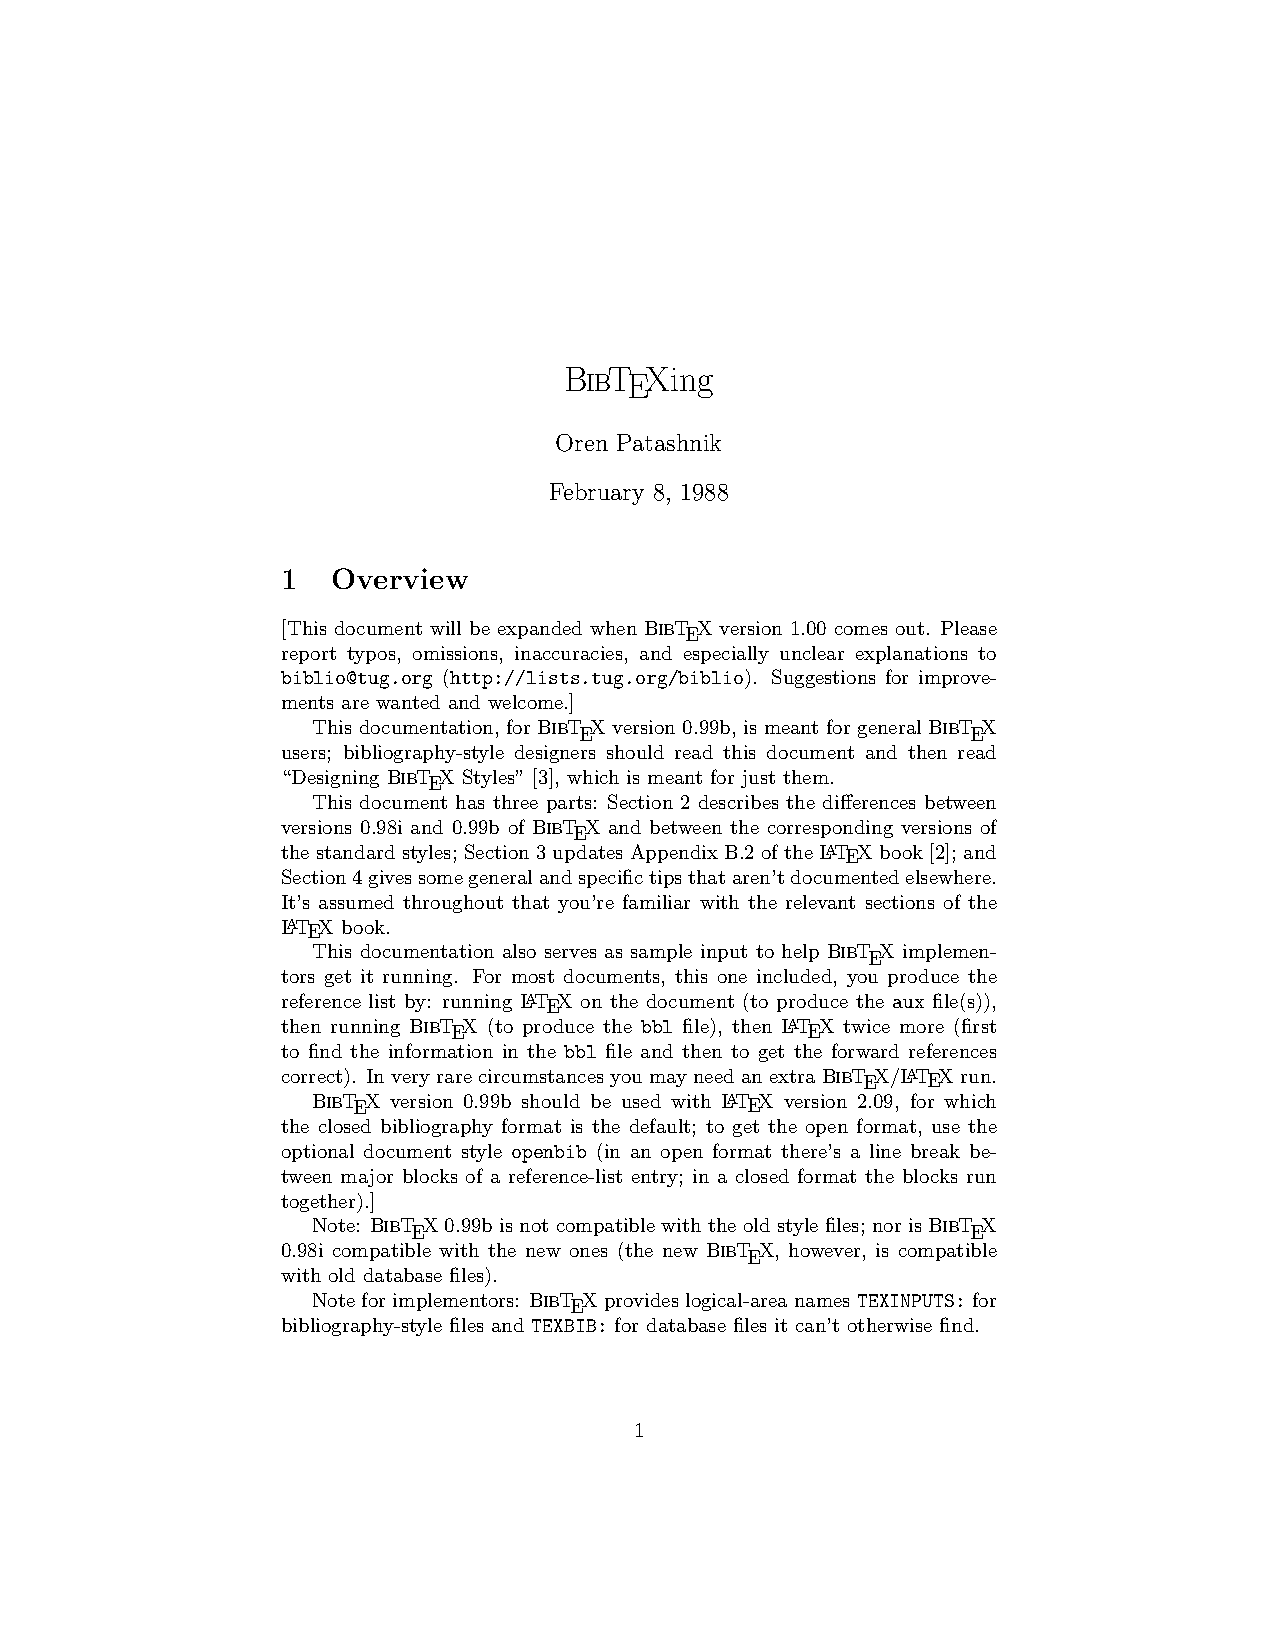
\includepdf[pages=1-3]{materials/bibTeX_intro.pdf}
\end{verbatim}
For more info see \url{http://en.wikibooks.org/wiki/LaTeX/Modular_Documents#Inserting_PDF_files}\\



%end of samples
\newpage %this command enforces the creation of a new page

%
%
% Zusammenfassungs-Segement (the geman version of the abstract) uncomment the content of this segment to use it:
%
% Remember: if you write in german, you must write a german AND an english abstract. If you write in english, including only an english abstract will suffice.
%

%\begin{center}
%{\LARGE Zusammenfassung}
%\end{center}

%Platz für Ihren Text
%\newpage %this command enforces the creation of a new page

%
%
% end of Zusammenfassungs-Segement 
%
%



\setcounter{page}{1}
\pagenumbering{arabic}
\hypersetup{pageanchor=true}

%put your Content after this marker
\part{Introduction}
Color is a property that is possessed by an object. The perception of color is nothing but our response to the combination of light, object and observer \citep{levkowitz1997color}. Even if one of these properties are removed then there will be no perception of color. Thus in order to understand color, it is important to also learn about the properties associated with an object. 
\\
\\
\noindent It is also important that the development of visual technologies are closely related to the human visual capabilities \citep{levkowitz1997color}. The most popular display devices used today, for example, CRT and flat screens, are not able to produce the same display quality of that photograph. This is due to the limitations in the spatial resolution for providing the same photograph\citep{levkowitz1997color}. Similar limitations can also be noted in the color domain due to the incompatible color gamuts used in the display device \citep{levkowitz1997color}. Thus, color modelling is still a research topic till date which can help provide cross-compatibility of colors \citep{levkowitz1997color}. 
\\
\\
Human eye consists of several components. The \textit{pupil} manages the amount of light admitted to the eye \citep{levkowitz1997color}. The \textit{cornea} is fixed and adapts the distance of the object from the observer. The retina performs "image processing" for our visual system and in addition to this, there are three types of cones present in the retina which also perform the filtering of different wavelengths as \textbf{Long, Medium and Short wavelength cones.} 
\\
\\
Color comprises of 3 aspects: \textbf{Hue, Saturation and Lightness.} \textit{Hue}, defines the actual color, \textit{Saturation}, defines how dark or bright a color is and \textit{Lightness} is associated with the amount of black mixed in a color. Even if any one of these three aspects are absent from an object, the color of the object cannot be perceived. 
\\
\\
Color models are given most importance when it comes to digital representation of colors, graphics or images. Some of the popular color models in the digital world are RGB, CMYK, HSL, etc. But RGB color space is commonly used in display technology. When it comes to human visualization, the RGB color space render colors that is not friendly to the visual mechanism of the human eye. Thus researchers suggest for using other color spaces that are present such as the LUV and the LMS color space. These color spaces are best suited for the human perception of colors.
\\
\\
Colors can also play an important role in the business world. Different color mean different to individuals. Thus it is very crucial to select the right color palette when it come to data visualization irrespective of whether data is represented by charts or plain data. The color tone used for representing data conveys information to the user. Colors also create an impact for web and desktop application.Thus selection of ideal color palette in business application is also critical.
\\
\\
The goal for this thesis topic is to create awareness on the importance of use of colors for designers are developers during the process of software or business report creation.





\pagebreak
\part{Visual perception}
The ability to collect information by observing the environment in visible light is called visual perception and visual system can be defined as a collective physiological parts that are responsible for enable visual perception.



\section{A big section}


\subsection{A subsection}

\subsubsection{A subsubsection}


\section{Another big section}



\pagebreak
\part{Conclusion and Outlook}

\section{A big section}




\pagebreak
\part{End Material}

\addcontentsline{toc}{section}{Material}

%
%
% start of material segment:
%
%

% remember: you can also include PDF-pages (see the samples above)

%
%
% end of material-segment
%
%


%After this line you should only change the naming of some parts or uncomment some lines where a comment gives you an explaination what to do. You should only change the structure and content beyond this point if you're sure you know what you're doing TeX-wise

\pagebreak
\addcontentsline{toc}{section}{List of Figures}%Creates an Entry in the table of contents without giving this a chapter number (looks more neat)
\listoffigures

\pagebreak
\addcontentsline{toc}{section}{List of Tables}%Creates an Entry in the table of contents without giving this a chapter number (looks more neat)
\listoftables

\pagebreak
\listoftheorems

%\renewcommand*{\glspostdescription}{}
%uncoment the previous line to get rid of the dot at the end of the description in the glossary

\pagebreak
\addcontentsline{toc}{section}{Abbreviations}%Creates an Entry in the table of contents without giving this a chapter number (looks more neat)
\printglossary[type=\acronymtype] % prints just the list of acronyms

\pagebreak
\addcontentsline{toc}{section}{Glossary}%Creates an Entry in the table of contents without giving this a chapter number (looks more neat)
\printglossary % full glossary


\addcontentsline{toc}{section}{Bibliography}%Creates an Entry in the table of contents without giving this a chapter number (looks more neat)

\nocite{*}%comment out this line if you don not wish to automatically include all entries from the thesis-bibliography
\bibliographystyle{apa}
\bibliography{./biblio/thesis}

\end{document}